\documentclass[aspectratio=169, plain, 14pt]{beamer}
\beamertemplatenavigationsymbolsempty
\setbeamertemplate{footline}[frame number]
\usepackage[utf8]{inputenc}
\usepackage[russian]{babel}
\usepackage[table]{xcolor}
\setbeamertemplate{itemize items}[circle]
\usepackage{ragged2e}
\usepackage{mathtools}
\usepackage{cleveref}
\usepackage{physics}

%My blocks
\setbeamercolor{block title}{fg=white,bg=blue!65!black}
\setbeamercolor{block body}{fg=black,bg=blue!10!white}
%%%%%%%%%%%%%%%%%%%%%%%%%%%%%%%%%%%

\title{Л6. Модель датчиков ЛА}
\author{Сутурин Даниил}
\institute{ЦНИИХМ}
\date{\today}

\begin{document}
	
	\begin{frame}
		\titlepage{}
	\end{frame}
	
	\begin{frame}{Откуда брать измерения?}
		\justifying\small
		\begin{columns}
			\column{0.7\linewidth}
			\begin{figure}
				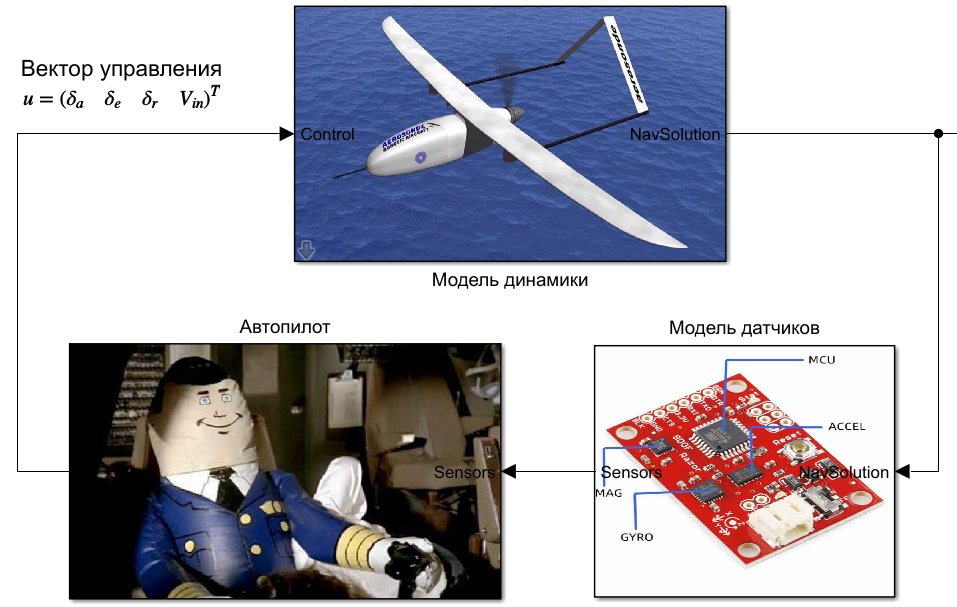
\includegraphics[width=0.95\textwidth]{DynMdl.png}
			\end{figure}
			\column{0.3\linewidth}
			Знаем как ведет ЛА в среде.
			\begin{itemize}
				\item Как управлять?
				\item Чем?
				\item На основе каких показаний?
			\end{itemize}
		\end{columns}
	\end{frame}
	
	\begin{frame}{Бортовое оборудование}
		\justifying\small
		\begin{columns}
			\column{0.61\linewidth}
			\begin{figure}
				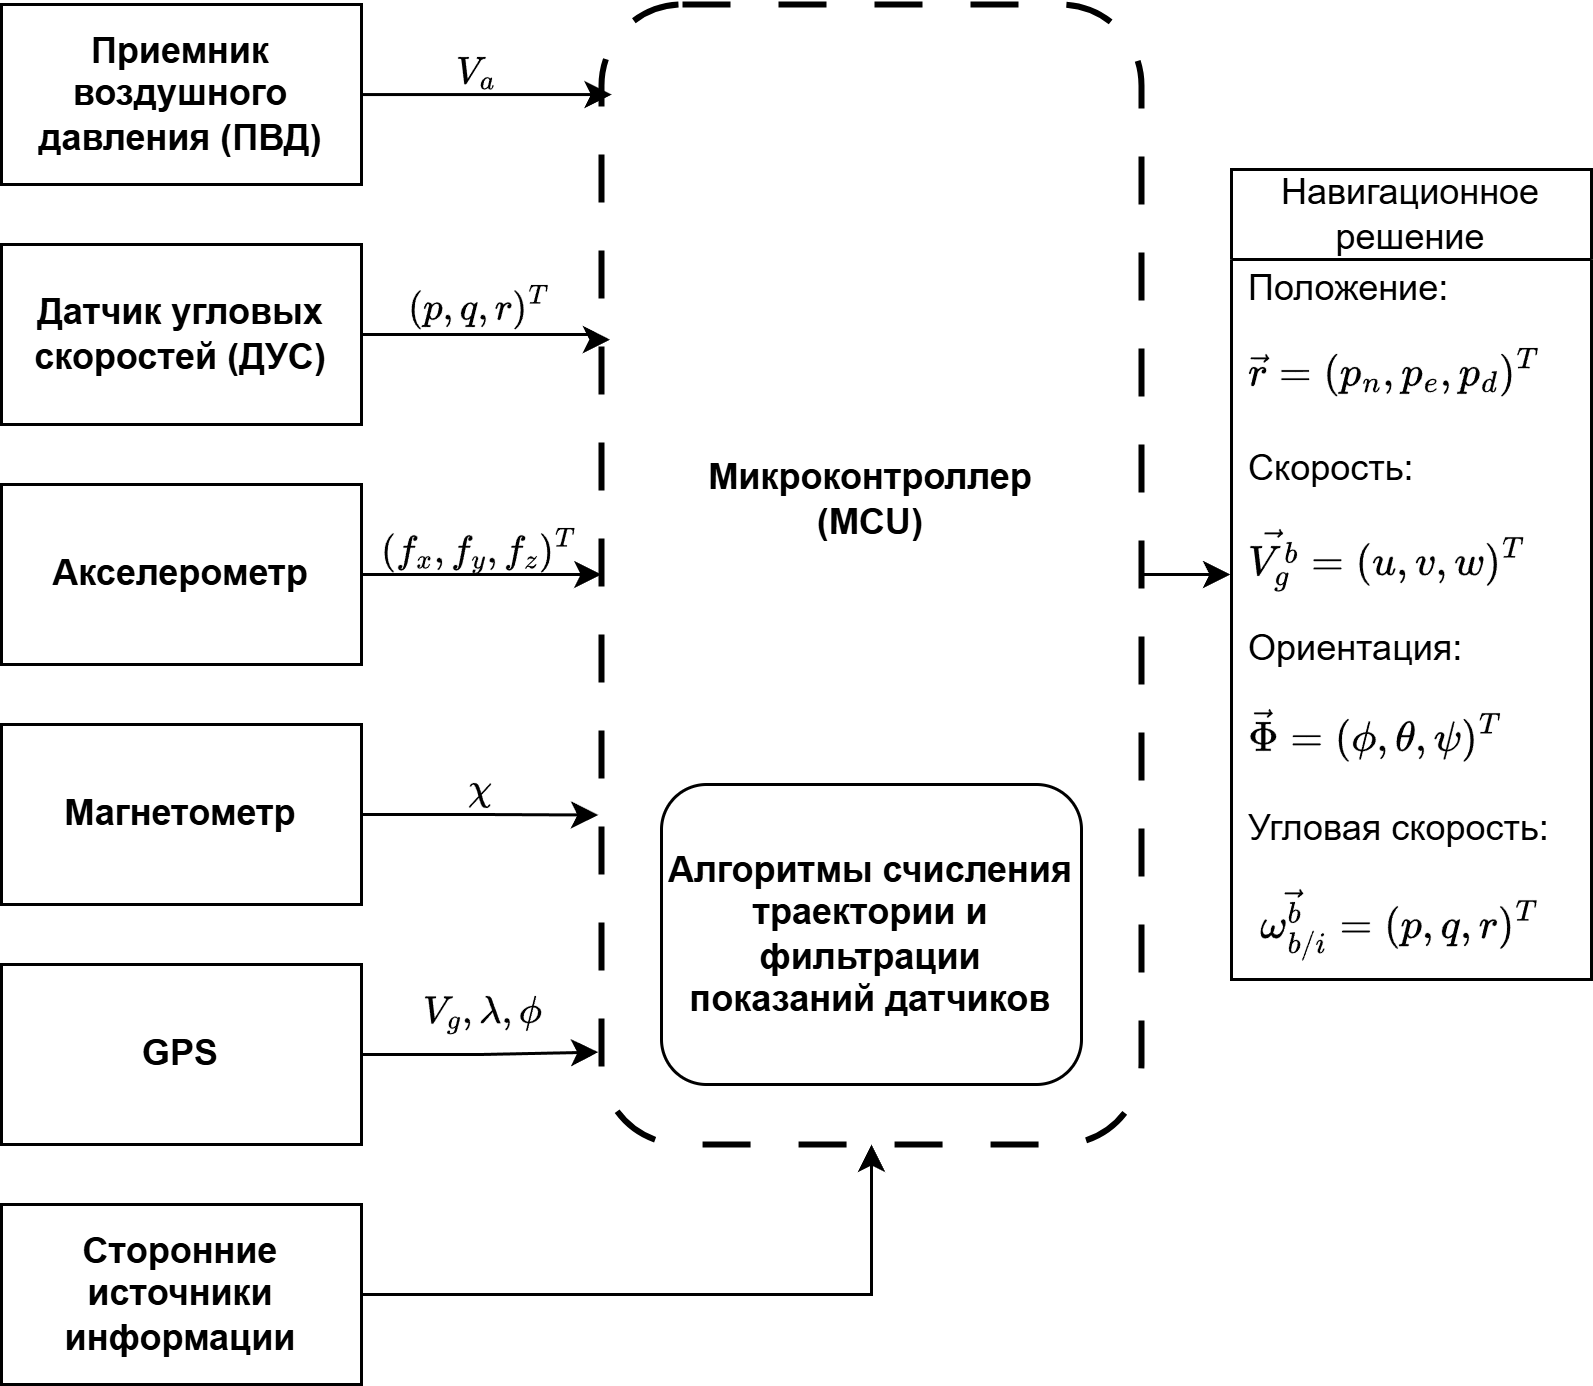
\includegraphics[width=1\textwidth]{SensorsDiagramm.png}
			\end{figure}
			\column{0.39\linewidth}
			\begin{figure}
				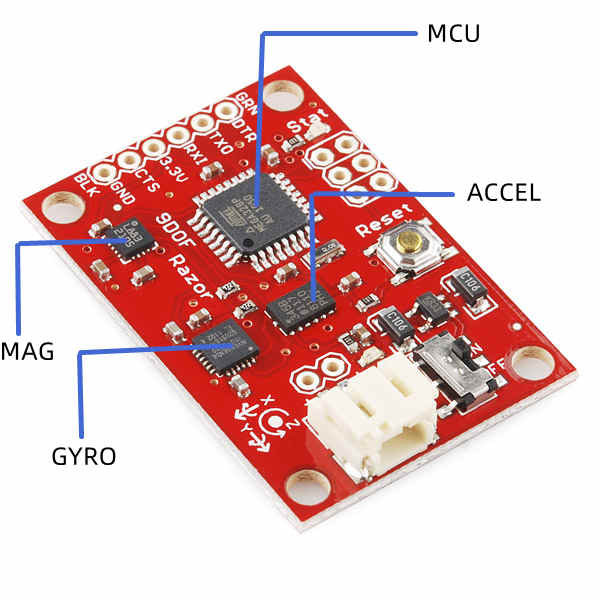
\includegraphics[width=1\textwidth]{IMU.jpg}
			\end{figure}
		\end{columns}
	\end{frame}
	
	\begin{frame}{Блок чувствительных элементов}
		\justifying\small
		Блок чувствительных элементов (Inertial Measurement Unit (IMU)) сочетает в себе \textbf{акселерометры} и датчики угловых скоростей (\textbf{ДУС}). Измеряет удельные силы и угловые скорости без информации извне о среде. Датчики, измеряющие угловые и линейные скорости и ускорения относительно некоторых выделенных объектов инерциальными не являются. 
		\begin{columns}
			\column{0.5\linewidth}
			\begin{figure}
				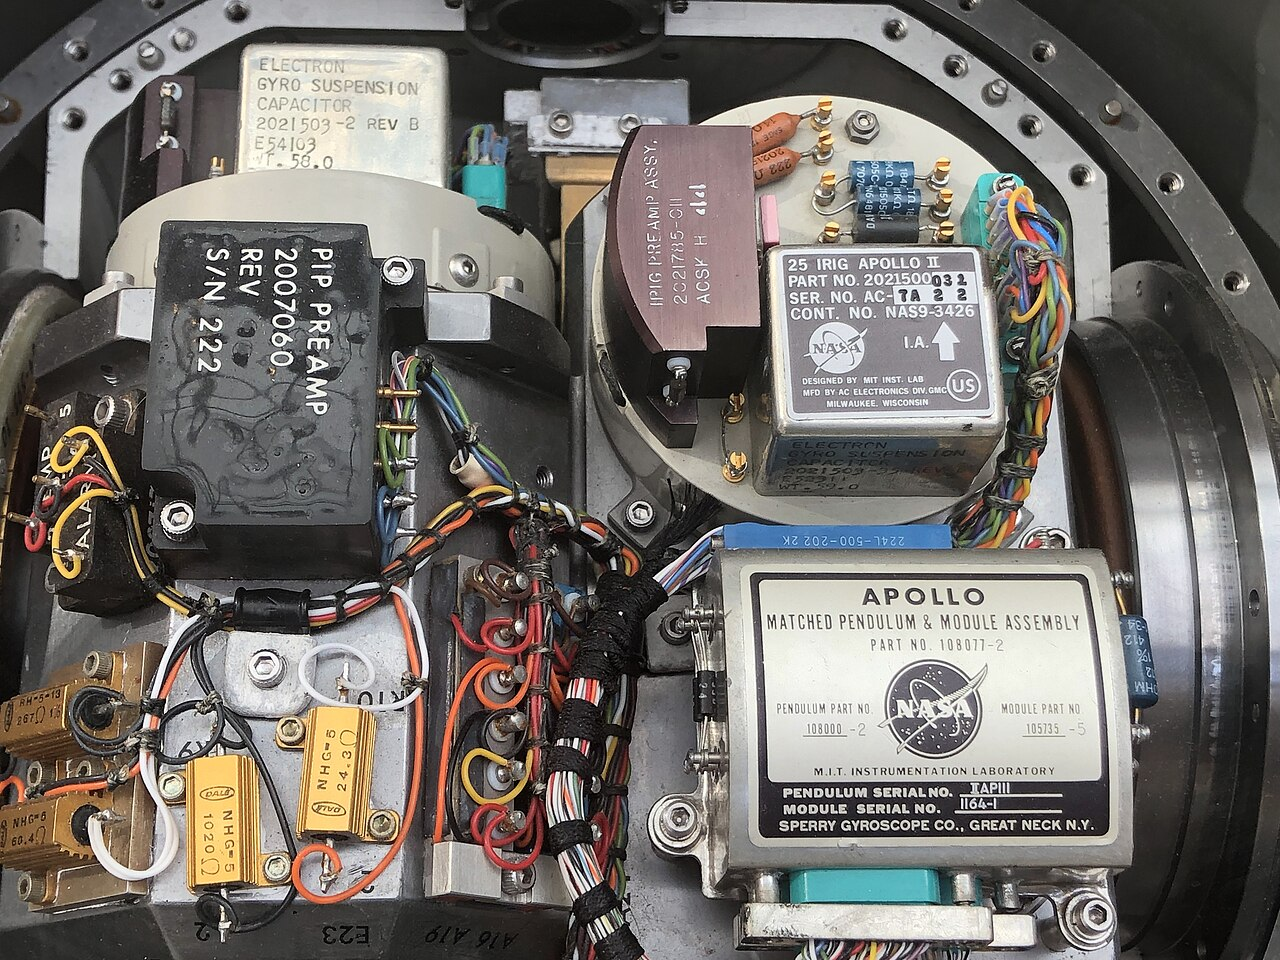
\includegraphics[width=0.75\textwidth]{Appolo_IMU.jpg}
				\caption{Инерциальный блок "Аполлона"}
			\end{figure}
			\column{0.5\linewidth}
			\begin{figure}
				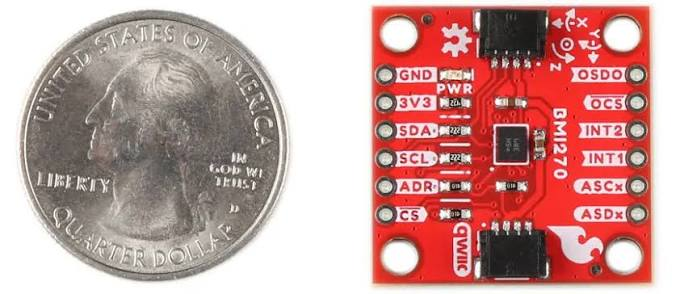
\includegraphics[width=0.8\textwidth]{CoinIMU.jpg}
				\caption{Современный микроэлектромеханический (МЭМС) БЧ}
			\end{figure}
		\end{columns}
	\end{frame}
	
	\begin{frame}{Акселерометр}
		\only<1>{
			\justifying\small
			\begin{columns}
				\column{0.5\linewidth}
				\begin{figure}
					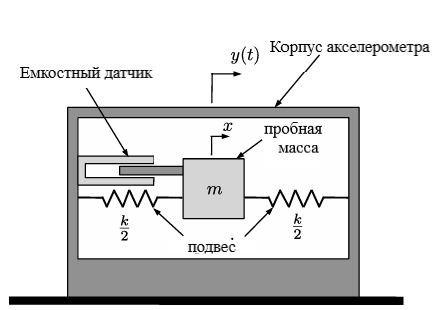
\includegraphics[width=0.9\textwidth]{Acc_scheme.png}
					\caption{Принцип работы акселерометра}
				\end{figure}
				\column{0.5\linewidth}
				\begin{figure}
					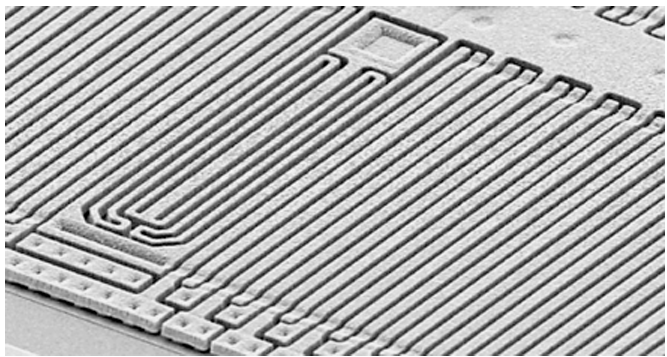
\includegraphics[width=0.9\textwidth]{Acc_mems.png}
					\caption{Внутренняя структура мэмс акселерометра}
				\end{figure}
			\end{columns}
			\begin{equation*}
				m\ddot{x}+kx=ky(t), \quad \ddot{x} = \frac{k}{m}\delta
			\end{equation*}
			Ускорение пробной массы пропорционально сжатию подвеса
		}
		
		%%%%%%%%%%%%%%%%%%%%%%%%%%%%%%%%%%%%%%%%%%
		\only<2>{
			\justifying\small
			Показания акселерометра можно смоделировать следующим образом:
			\begin{equation*}
				\boldsymbol{y}_{acc}^{'} = k_{acc}\boldsymbol{A} + \boldsymbol{\beta}_{acc} + \boldsymbol{\eta}_{acc},
			\end{equation*}
			\begin{itemize}
				\item $\boldsymbol{y}_{acc}^{'}$ - напряжение с емкостного датчика
				\item $k_{acc}$ - коэффициент пропорциональности $\frac{\text{м/}\text{с}^2}{\text{В}}$ (из документации)
				\item A - ускорение $\frac{\text{м}}{\text{с}^2}$
				\item $\boldsymbol{\beta}_{acc}$ - смещение нуля
				\item $\eta_{acc}$ - случайный шум (обычно Гауссовый $\mu_{acc} = 0$, $\sigma_{acc} \neq 0$)
			\end{itemize}
		}
		
		%%%%%%%%%%%%%%%%%%%%%%%%%%
		\only<3>{
		\justifying\small
		Акселерометр измеряет удельные силы. В состоянии покоя в поле тяготения показания будут ненулевые равные $\boldsymbol{g}$. Поэтому кажущиеся ускорения равны показаниям акселерометра минус ускорение свободного падения:
		\begin{equation*}
			\boldsymbol{y}_{acc}^{'} = k_{acc}R_b^a\left(\frac1m\boldsymbol{f}^b - R_i^b\boldsymbol{g} + \boldsymbol{\beta}_{acc} + \boldsymbol{\eta}_{acc} \right),
		\end{equation*}
		$R_b^a$ - матрица перехода из чувствительных осей акселерометра в ССК
		
		Коэффициент пропорциональности $k_{acc}$ и $R_b^a$ определяются на этапе калибровки на земле, тогда:
 		\begin{equation*}
		 	\boldsymbol{y}_{acc} = \frac{1}{k_{acc}}R_a^b\boldsymbol{y}_{acc}^{'} =  \frac1m\boldsymbol{f}^b - R_i^b\boldsymbol{g} + \boldsymbol{\beta}_{acc} + \boldsymbol{\eta}_{acc},
		 \end{equation*}
		}
		%%%%%%%%
		\only<4>{
			\justifying\small
			Согласно уравнениям движения из прошлых лекций линейные ускорения в ССК:
			\begin{equation*}
				\boldsymbol{f}^{b} = m\left(\frac{d\boldsymbol{V}}{dt_b} + \boldsymbol{\omega}_{b/i}^b\times\boldsymbol{V}\right) 
			\end{equation*}
			Тогда показания акселерометров $y_{acc} = (a_x \quad a_y \quad a_z)^T$:
			
			$$
			a_x = \dot{u} + qw -rv + g\sin{\theta} + \beta_{acc,x} + \eta_{acc,x}
			$$
			
			$$
			a_y = \dot{v} + ru -pw - g\cos{\theta}\sin{\phi} + \beta_{acc,y} + \eta_{acc,y}
			$$
			
			$$
			a_z = \dot{w} + pv -qu -g\cos{\theta}\cos{\phi} + \beta_{acc,z} + \eta_{acc,z}
			$$
			
		}
	\end{frame}
	
	%%%%%%%%%%%%%%%%%%%%%%%%%%%%%%%%%%%%%%
	\begin{frame}{Датчик угловых скоростей}
		\only<1>{
		\justifying\small
			\begin{figure}
				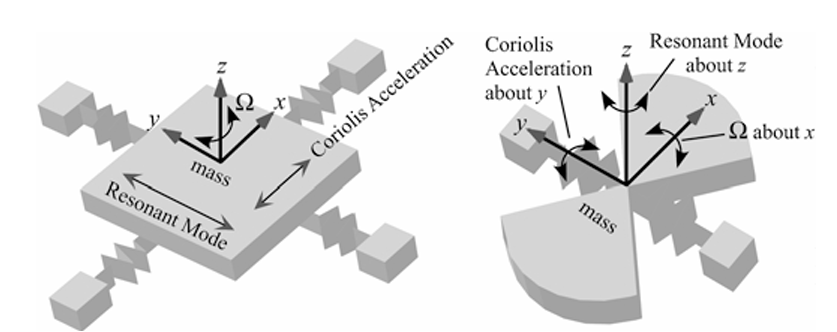
\includegraphics[width=0.7\textwidth]{Gyro_scheme.png}
				\caption{Принцип работы ДУС}
			\end{figure}
			Действие ДУС основано на эффекте Кориолисова ускорения $\boldsymbol{a}_c = 2\boldsymbol{\Omega}\times\boldsymbol{V}$
		}
		
		%%%%%%%%%%%%%%%%%%%%%%%%%%%%%
		\only<2>{
			\justifying\small
		Пробная масса совершает колебания $V = A\omega_n\sin{\omega_nt}$. При возникновении вращения $\boldsymbol{\Omega}$ ДУС в ортогональной плоскости на пробную массу оказывает воздействие Кориолисово ускорение $\boldsymbol{a}_c$. Ускорение измеряется емкостным датчиком по аналогии с акселерометром:
		$V_{gyr} = k|\boldsymbol{a}_c| = 2k\Omega A\omega_n = K\Omega$
		
		$$\boldsymbol{y}_{gyr}^{'} = k_{gyr}\boldsymbol{\Omega} + \boldsymbol{\beta}_{gyr} + \boldsymbol{\eta_{gyr}},$$
		\begin{itemize}
			\item $\boldsymbol{y}_{gyr}^{'}$ - напряжение с емкостного датчика
			\item $k_{gyr}$ - коэффициент пропорциональности $\frac{\text{рад/}\text{с}}{\text{В}}$ (из документации)
			\item $\boldsymbol{\Omega}$ - угловая скорость $\frac{\text{рад}}{\text{с}}$
			\item $\boldsymbol{\beta}_{gyr}$ - смещение нуля
			\item $\eta_{gyr}$ - случайный шум (обычно Гауссовый $\mu_{gyr} = 0$, $\sigma_{gyr} \neq 0$)
		\end{itemize}
		}
		
		%%%%%%%%%%%%%%%%%%%%%%%%%
		\only<3>{
			По аналогии с акселерометром коэффициент пропорциональности $k_{gyr}$ и матрица перехода из чувствительных осей ДУС в ССК $R_{g}^{b}$ определяются на этапе калибровки. Тогда показания ДУС имеют вид:
			$$\boldsymbol{y}_{gyr}^{'} = k_{gyr}R_{b}^{g}\left(\boldsymbol{\omega}_{b/i}^{b} + \boldsymbol{\beta}_{gyr} + \boldsymbol{\eta}_{gyr} \right) $$
			
			$$
			\boldsymbol{y}_{gyr} = \frac{1}{k_{gyr}}R_{g}^{b}\boldsymbol{y}_{gyr}^{'} = \boldsymbol{\omega}_{b/i}^{b} + \boldsymbol{\beta}_{gyr} + \boldsymbol{\eta}_{gyr}
			$$
			
			$$\omega_x = p + \beta_{gyr,x} + \eta_{gyr,x}$$
			$$\omega_y = q + \beta_{gyr,y} + \eta_{gyr,y}$$
			$$\omega_z = r + \beta_{gyr,z} + \eta_{gyr,z}$$
		}
	\end{frame}
	
	%%%%%%%%%%%%%%%%%%%%%%%
	\begin{frame}{Бародатчик}
		\justifying\small
		\begin{columns}
			\column{0.5\linewidth}
			\begin{figure}
				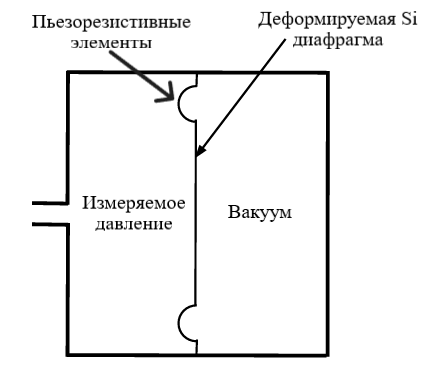
\includegraphics[width=0.9\textwidth]{Press.png}
				\caption{Принцип работы бародатчика}
			\end{figure}
			\column{0.5\linewidth}
			На небольших высотах изменение давление можно описать барометрической формулой:
			$$P(h) = P_0e^{-\frac{\mu g}{RT(h)}h}$$
			Тогда показания датчика абсолютного давления:
			$$z_{pres} = \rho g h + \beta_{pres} + \eta_{pres}$$
		\end{columns}

	\end{frame}
	
	\begin{frame}{Приемник воздушного давления}
		\justifying\small
			\begin{figure}
				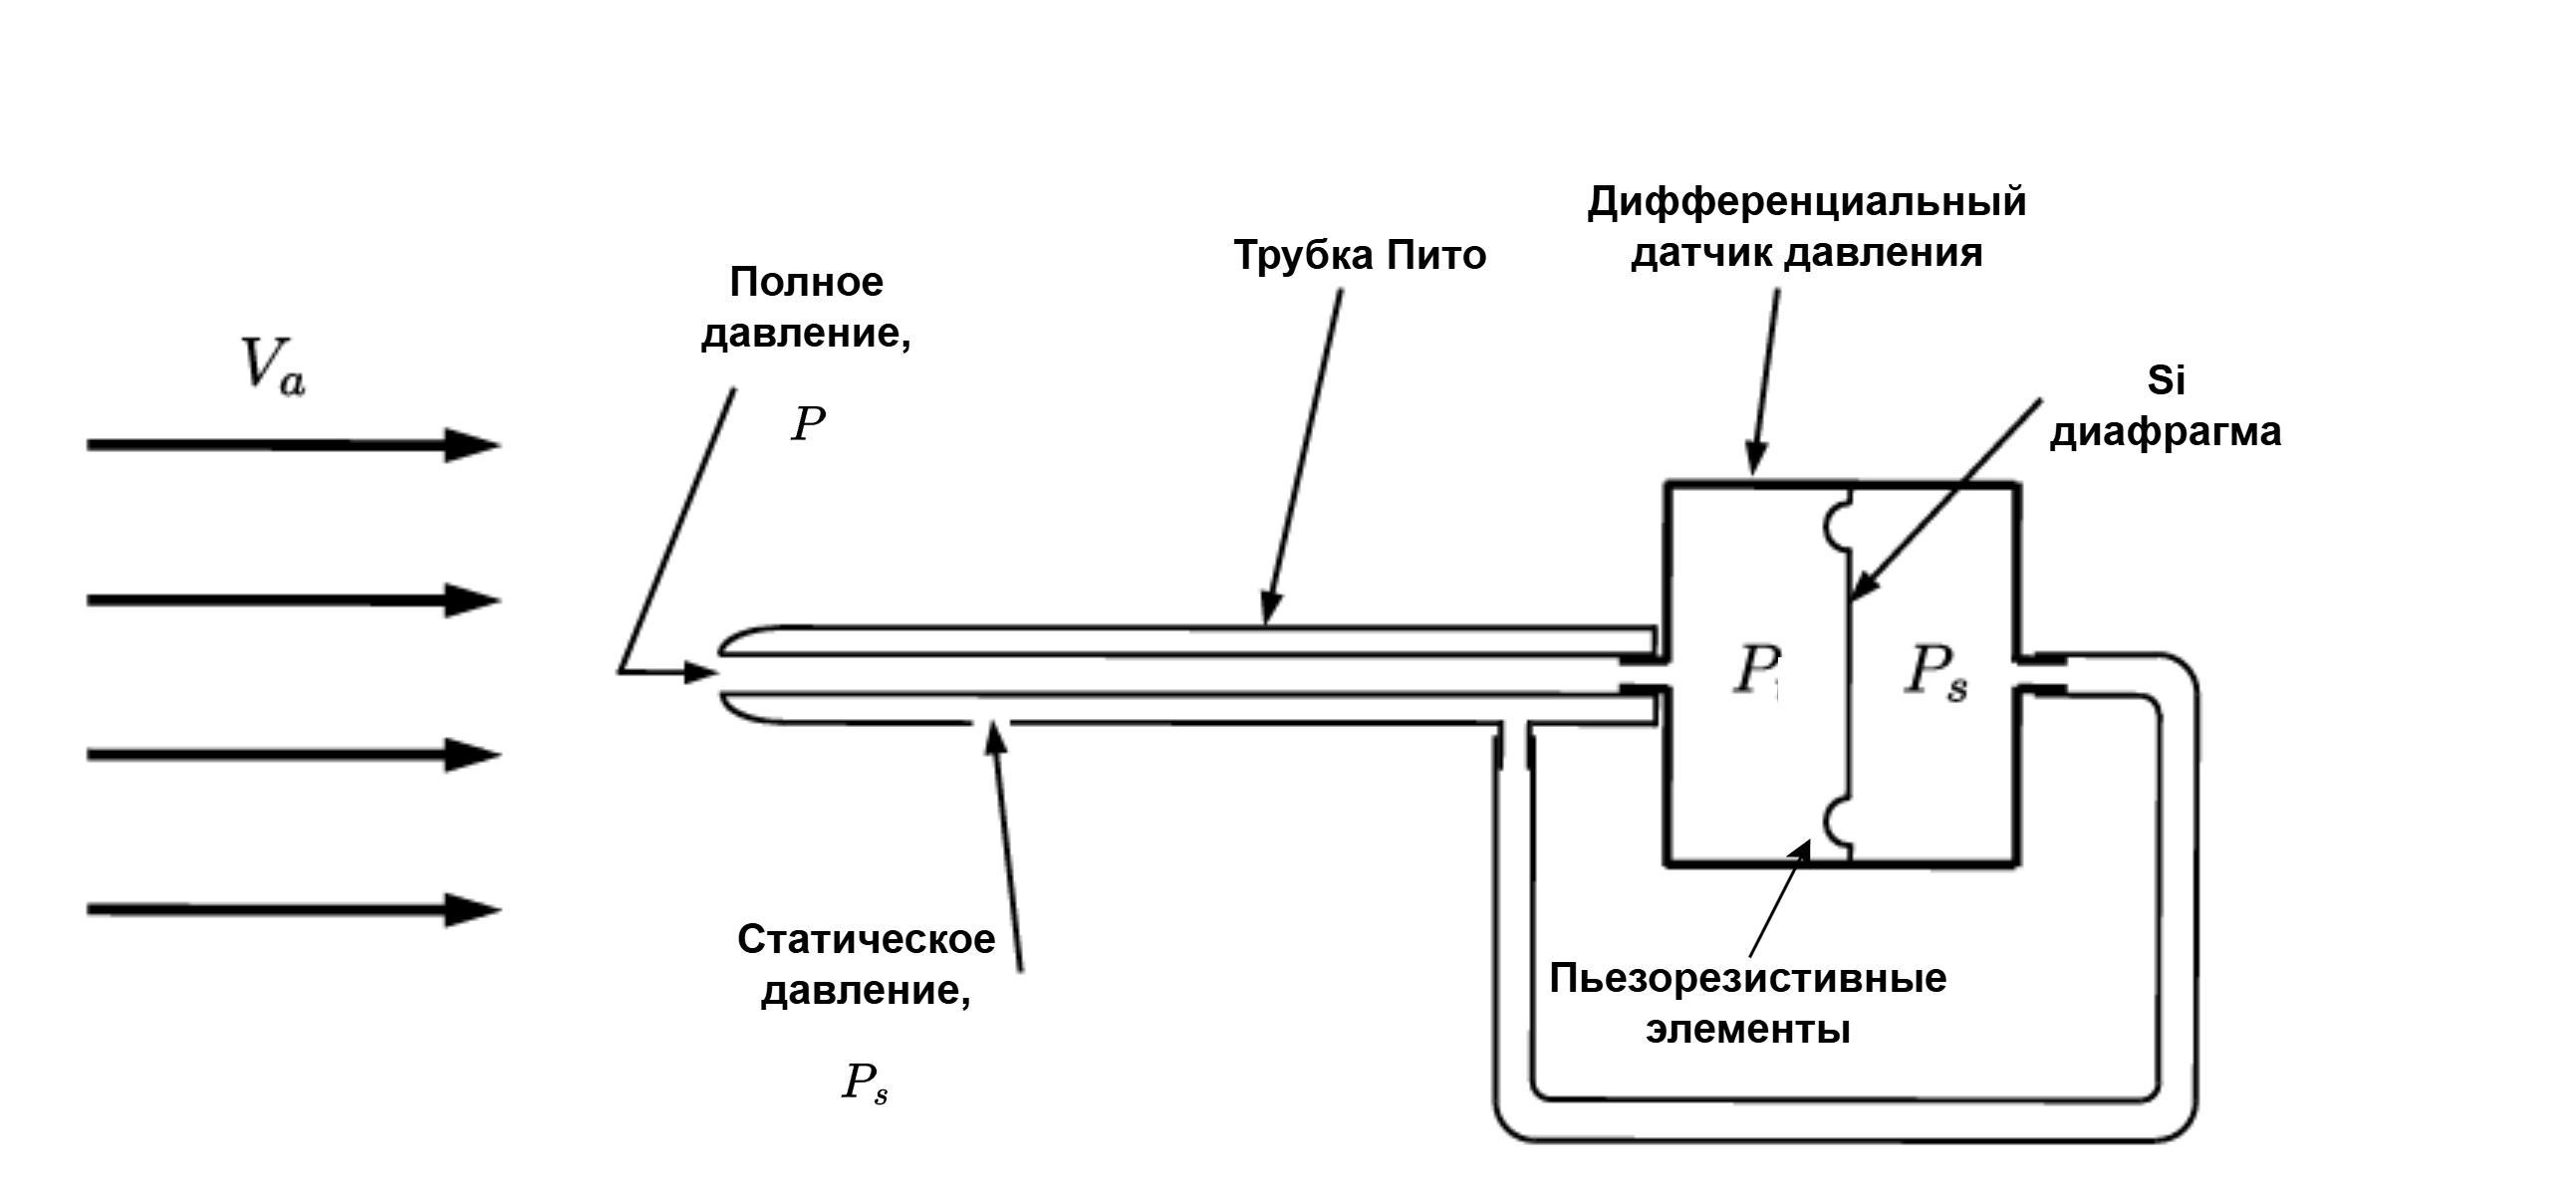
\includegraphics[width=0.7\textwidth]{ASPD_scheme.png}
				\caption{Принцип работы ПВД}
			\end{figure}
			Полное давление - сумма сатического и динамического:
			$$P = P_s + \frac{\rho V_{a}^2}{2}, \quad z_{aspd} = \frac{\rho V_{a}^2}{2} + \beta_{aspd} + \eta_{aspd}$$
	\end{frame}
	
	%%%%%%%%%%%%%%%%%%%%%%%%%%%%%%%%%%%%%%
	\begin{frame}{Технологии производства МЭМС}
	\only<1>{
		\justifying\small
		Основной материал для микроэлектромеханических систем - кремний Si.
		\begin{itemize}
			\item 1954 г. описаны пъезорезистивные свойства Si и Ge ("Piezoresistance Effect in Germanium and Silicon" Smith, 1954)\\
			\item конец 1950-х коммерческая разработка кремниевых тензодатчиков \\
			\item 1970-е годы - методы механической и химической обработки кремниевых подложек для миниатюрных, гибких МЭМС \\
			\item 1980-е годы - создание интегральных микросхем на основе Si \\ 
		\end{itemize}
	}	
	
	%%%%%%%%%%%%%%%%%%%%%%%%%%%%%%%
	\only<2>{
	Кремний один из самых распространенных элементов земной коры. Процесс получения многостадийный, науко- и энергоемкий
	\begin{figure}
		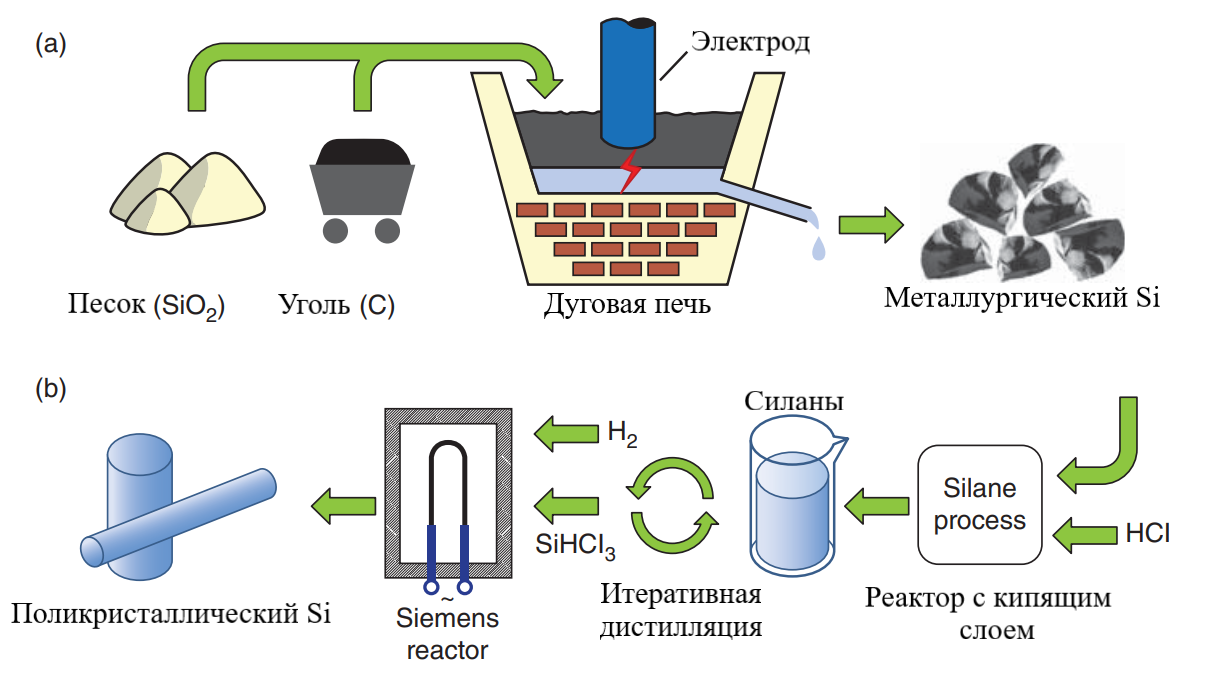
\includegraphics[width=0.8\textwidth]{Si_production1.png}
	\end{figure}
	}
	%%%%%%%%%%%%%%%%%%%%%%%%%%%%%%%%%%%
	\only<3>{
	\begin{figure}
		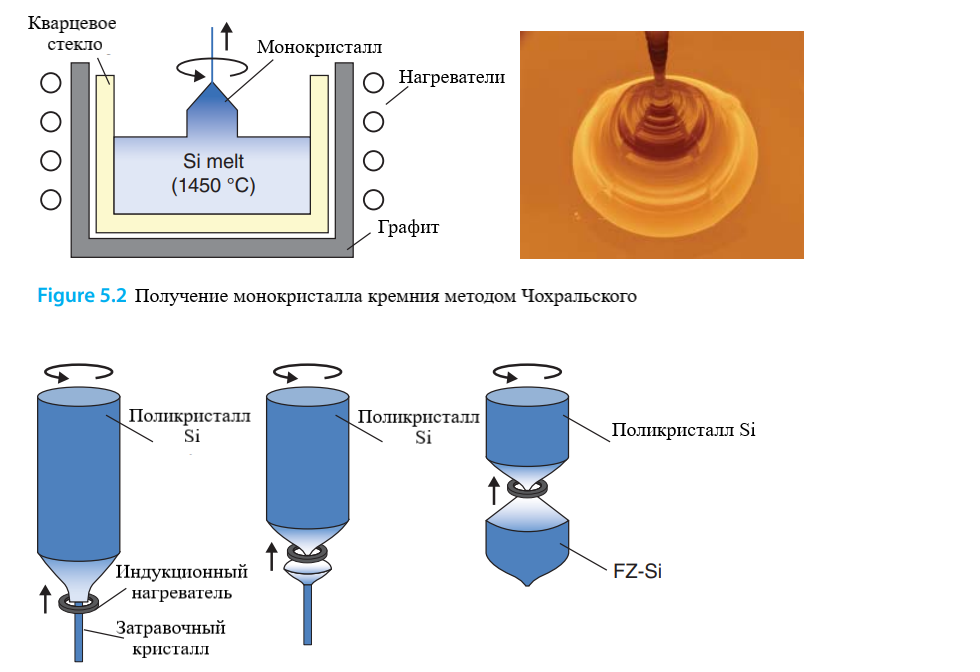
\includegraphics[width=0.8\textwidth]{Si_production11.png}
	\end{figure}
	}
	%%%%%%%%%%%%%%%%%%%%%%%%%%%%%%%%%%%%%
	\only<4>{
	\begin{figure}
		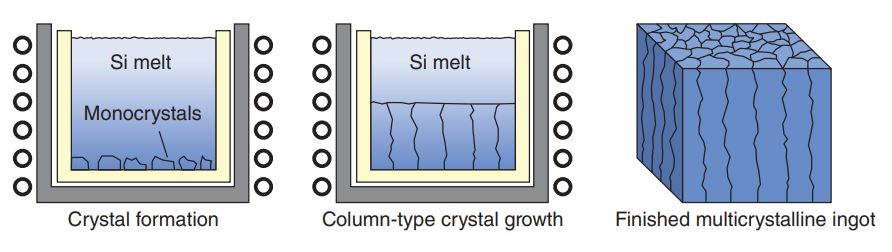
\includegraphics[width=1\textwidth]{Si_production2.png}
	\end{figure}
	}
	%%%%%%%%%%%%%%%%%%%%%%%%%%%%%%%%%%%%%
	\only<5>{
		\begin{figure}
			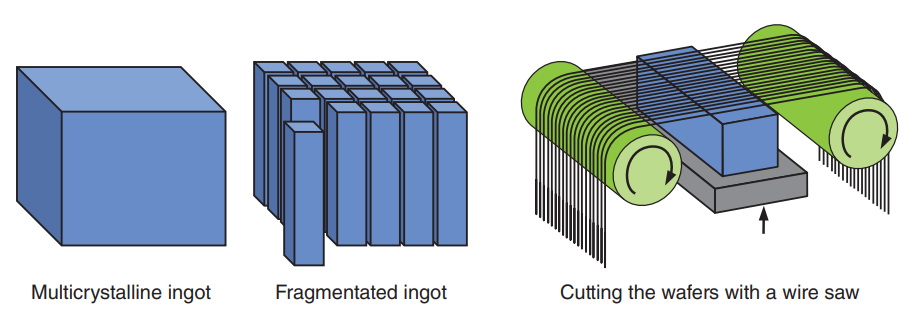
\includegraphics[width=1\textwidth]{Si_production3.png}
		\end{figure}
	}
	%%%%%%%%%%%%%%%%%%%%%%%%%%%%%%%%%%%%%
	\only<6>{
		\begin{figure}
			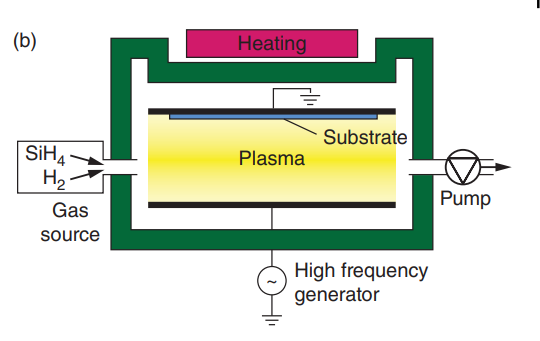
\includegraphics[width=0.75\textwidth]{Si_production4.png}
			\caption{Плазменно-химическое осаждение из газовой фазы}
		\end{figure}
	}
	\end{frame}
\end{document}